\documentclass[portrait,final,archA0,fontscale=0.372]{baposter}

\usepackage{etoolbox}
\patchcmd{\thebibliography}{\section*{\refname}}{}{}{}
\usepackage{calc}
\usepackage{graphicx}
\usepackage{amsmath}
\usepackage{amssymb}
\usepackage{relsize}
\usepackage{multirow}
\usepackage{rotating}
\usepackage{bm}
\usepackage{url}
\usepackage{color}

\usepackage{graphicx}
\usepackage{multicol}

%\usepackage{times}
%\usepackage{helvet}
%\usepackage{bookman}
\usepackage{palatino}

\newcommand{\captionfont}{\footnotesize}

\setlength{\columnsep}{1.5em}
\setlength{\columnseprule}{0mm}


\newcommand{\compresslist}{%
\setlength{\itemsep}{1pt}%
\setlength{\parskip}{0pt}%
\setlength{\parsep}{0pt}%
}



\begin{document}


\definecolor{airforceblue}{rgb}{0.36, 0.54, 0.66}

%%
\begin{poster}%
  % Poster Options
  {
  % Show grid to help with alignment
  grid=false,
  % Column spacing
  colspacing=1em,
  % Color style
  bgColorOne=white,
  borderColor=green,
  headerColorOne=orange,
  headerColorOne=orange,
  headerFontColor=black,
  boxColorOne=white,
  % Format of textbox
  textborder=rectangle,
  % Format of text header
  eyecatcher=true,
  headerborder=closed,
  headerheight=0.1\textheight,
%  textfont=\sc, An example of changing the text font
  headershape=rectangle,
  headershade=shadelr,
  headerfont=\Large\bf\textsc, %Sans Serif
  textfont={\setlength{\parindent}{1.5em}},
  boxshade=plain,
%  background=shade-tb,
  background=plain,
  linewidth=2pt
  }
  % Eye Catcher
  {\begin{minipage}{8em}
   \hfill\vspace{1in}
  \end{minipage} } % Empty space, replace with image if desired
  % Title
  {\bf \textsc{  Measurement Device Independence \\ Eve's worst nightmare  } }
  % Authors
  {\textsc{  Chris Irish and Jonathan Gough \\ Department of Physics and Astronomy}}
  % University logo
  {% The makebox allows the title to flow into the logo, this is a hack because of the L shaped logo.
    
\includegraphics[height=9.0em]{img/ucl_logo}
  }

%%%%%%%%%%%%%%%%%%%%%%%%%%%%%%%%%%%%%%%%%%%%%%%%%%%%%%%%%%%%%%%%%%%%%%%%%%%%%%
%%% Now define the boxes that make up the poster
%%%---------------------------------------------------------------------------
%%% Each box has a name and can be placed absolutely or relatively.
%%% The only inconvenience is that you can only specify a relative position 
%%% towards an already declared box. So if you have a box attached to the 
%%% bottom, one to the top and a third one which should be in between, you 
%%% have to specify the top and bottom boxes before you specify the middle 
%%% box.
%%%%%%%%%%%%%%%%%%%%%%%%%%%%%%%%%%%%%%%%%%%%%%%%%%%%%%%%%%%%%%%%%%%%%%%%%%%%%%
    %
    % A coloured circle useful as a bullet with an adjustably strong filling
    \newcommand{\colouredcircle}{%
      \tikz{\useasboundingbox (-0.2em,-0.32em) rectangle(0.2em,0.32em); \draw[draw=black,fill=lightblue,line width=0.03em] (0,0) circle(0.18em);}}

%%%%%%%%%%%%%%%%%%%%%%%%%%%%%%%%%%%%%%%%%%%%%%%%%%%%%%%%%%%%%%%%%%%%%%%%%%%%%%
  \headerbox{Alice Has A Secret}{name=Alice Has A Secret,column=0,row=0}{
%%%%%%%%%%%%%%%%%%%%%%%%%%%%%%%%%%%%%%%%%%%%%%%%%%%%%%%%%%%%%%%%%%%%%%%%%%%%%%

\noindent\textbf{It started with a secret}. Alice "found" a wholesale box of Monster Munch behind the UCL cafeteria, and quickly stashed it in some bushes. She wanted to share it with Bob, as she'd never manage the entire box herself, but had to be careful, or she might have to share with everyone else too! She sent an \textbf{encrypted message} to Bob, to share the amazing news, but the joy would soon turn sour. Bob called back shortly afterwards - he'd been to the drop, but every one of the delectable maize snacks had vanished! They realised their secret \textbf{encryption key} had been cracked, and it could only be one person: \textbf{Eve the eavesdropper}. Eve loves to learn people's secrets and share them with everyone, and Alice is the perfect mark. Alice and Bob need a method to tell when Eve is listening in on their conversations, luckily Bob's been reading the latest issue of cryptographic weekly and thinks he may have the answer. They needed \textbf{Quantum Key Distribution}!

%Many encryption methods are based on maths problems that are too hard for computers to solve within a sensible time, but have solutions that can be quickly checked, making them quick to use, but hard to crack. But these methods were now vulnerable to new quantum computers, and Eve must have asked for one for her recent birthday!$ 

\begin{center}
    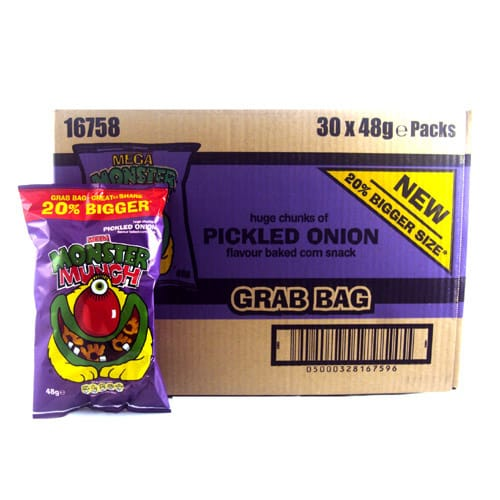
\includegraphics[width=0.75\linewidth]{img/mm} 
\end{center}


}

%%%%%%%%%%%%%%%%%%%%%%%%%%%%%%%%%%%%%%%%%%%%%%%%%%%%%%%%%%%%%%%%%%%%%%%%%%%%%%
  \headerbox{References}{name=references,column=0,above=bottom}{
%%%%%%%%%%%%%%%%%%%%%%%%%%%%%%%%%%%%%%%%%%%%%%%%%%%%%%%%%%%%%%%%%%%%%%%%%%%%%%

\bibliographystyle{unsrt} 
%\cite{PhysRevX.6.011024}$ 
\bibliography{references}

}

%%%%%%%%%%%%%%%%%%%%%%%%%%%%%%%%%%%%%%%%%%%%%%%%%%%%%%%%%%%%%%%%%%%%%%%%%%%%%%
  \headerbox{Quantum Key Distribution}{name=Quantum Key Distribution,column=0,below=Alice Has A Secret, above=references}{
%%%%%%%%%%%%%%%%%%%%%%%%%%%%%%%%%%%%%%%%%%%%%%%%%%%%%%%%%%%%%%%%%%%%%%%%%%%%%%

\noindent Luckily, UCL had some suitable components lying around, and a spare \textbf{fibre-optic network}, spanning important sites such as IT, the Library, and McDonald's. With QKD in place, Alice sent photons of light, polarised in different directions to represent binary bit values (0 or 1) of the \textbf{encryption keys}. They would switch their instruments randomly between two \textbf{bases}, so that if you measured in the wrong basis, you would get a random value, and you couldn't be sure if anything was correct. Eve's also been reading the latest issue though and is familiar with the dark arts of quantum hacking, and wouldn't be put off so easily. She intercepted and measured some of Alice's photons, and prepared new photons to send on to Bob. Alice and Bob were clever though. They shared some of the results on the phone, with Eve listening in, and managed to spot the wrong bits, or \textbf{bit errors}, caused when she'd guessed incorrectly.

\vspace{0.3cm}

\noindent Eve was rumbled, it seemed all was lost. But another flick through the latest cryptography weekly gave her new hope - she just had to be extra sneaky to exploit the \textbf{loopholes}. Alice's signal would experience interference from the environment, and the further it travelled, the more bit errors were introduced. Errors also occurred due to their equipment gradually starting to point the wrong way, or becoming misaligned. The errors caused by Eve's interactions became harder to spot. Eve learned to cleverly manipulate the signal to put Alice and Bob's equipment a little out of sync without them realising, providing extra cover for her attacks. Worse still, distances of over a few km, such as from the library to McDonald's, weren't possible without using a relay to pass on the signal. This relay Eve could easily hack, and control.

\vspace{0.3cm}

\noindent Even as Alice transmitted the entire contents of her little sister's diary, she didn't talk for fear of discovery. But when Alice confessed that her favourite Love Island contestant was Curtis, Eve just couldn't be quiet any longer, and humiliation soon followed.

}

%%%%%%%%%%%%%%%%%%%%%%%%%%%%%%%%%%%%%%%%%%%%%%%%%%%%%%%%%%%%%%%%%%%%%%%%%%%%%%
\headerbox{Map}{name=Map,column=1,span=2,row=0}{
%%%%%%%%%%%%%%%%%%%%%%%%%%%%%%%%%%%%%%%%%%%%%%%%%%%%%%%%%%%%%%%%%%%%%%%%%%%%%%

\begin{center}
    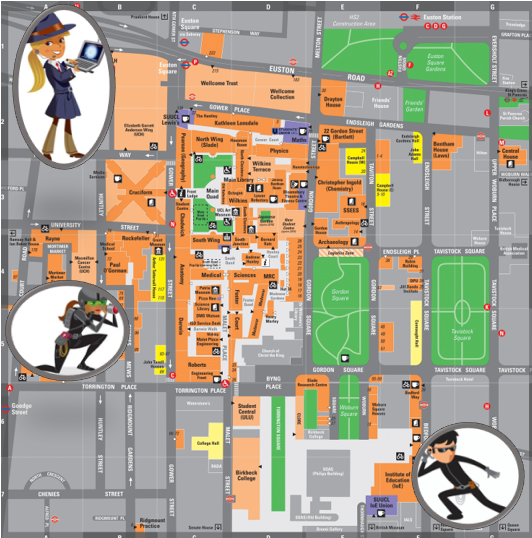
\includegraphics[width=\linewidth]{img/combined} 
\end{center}  

}

%%%%%%%%%%%%%%%%%%%%%%%%%%%%%%%%%%%%%%%%%%%%%%%%%%%%%%%%%%%%%%%%%%%%%%%%%%%%%%
  \headerbox{Definitions}{name=Definitions,column=1, span=2,below=Map }{
%%%%%%%%%%%%%%%%%%%%%%%%%%%%%%%%%%%%%%%%%%%%%%%%%%%%%%%%%%%%%%%%%%%%%%%%%%%%%%
\begin{multicols}{2}

\begin{center}
    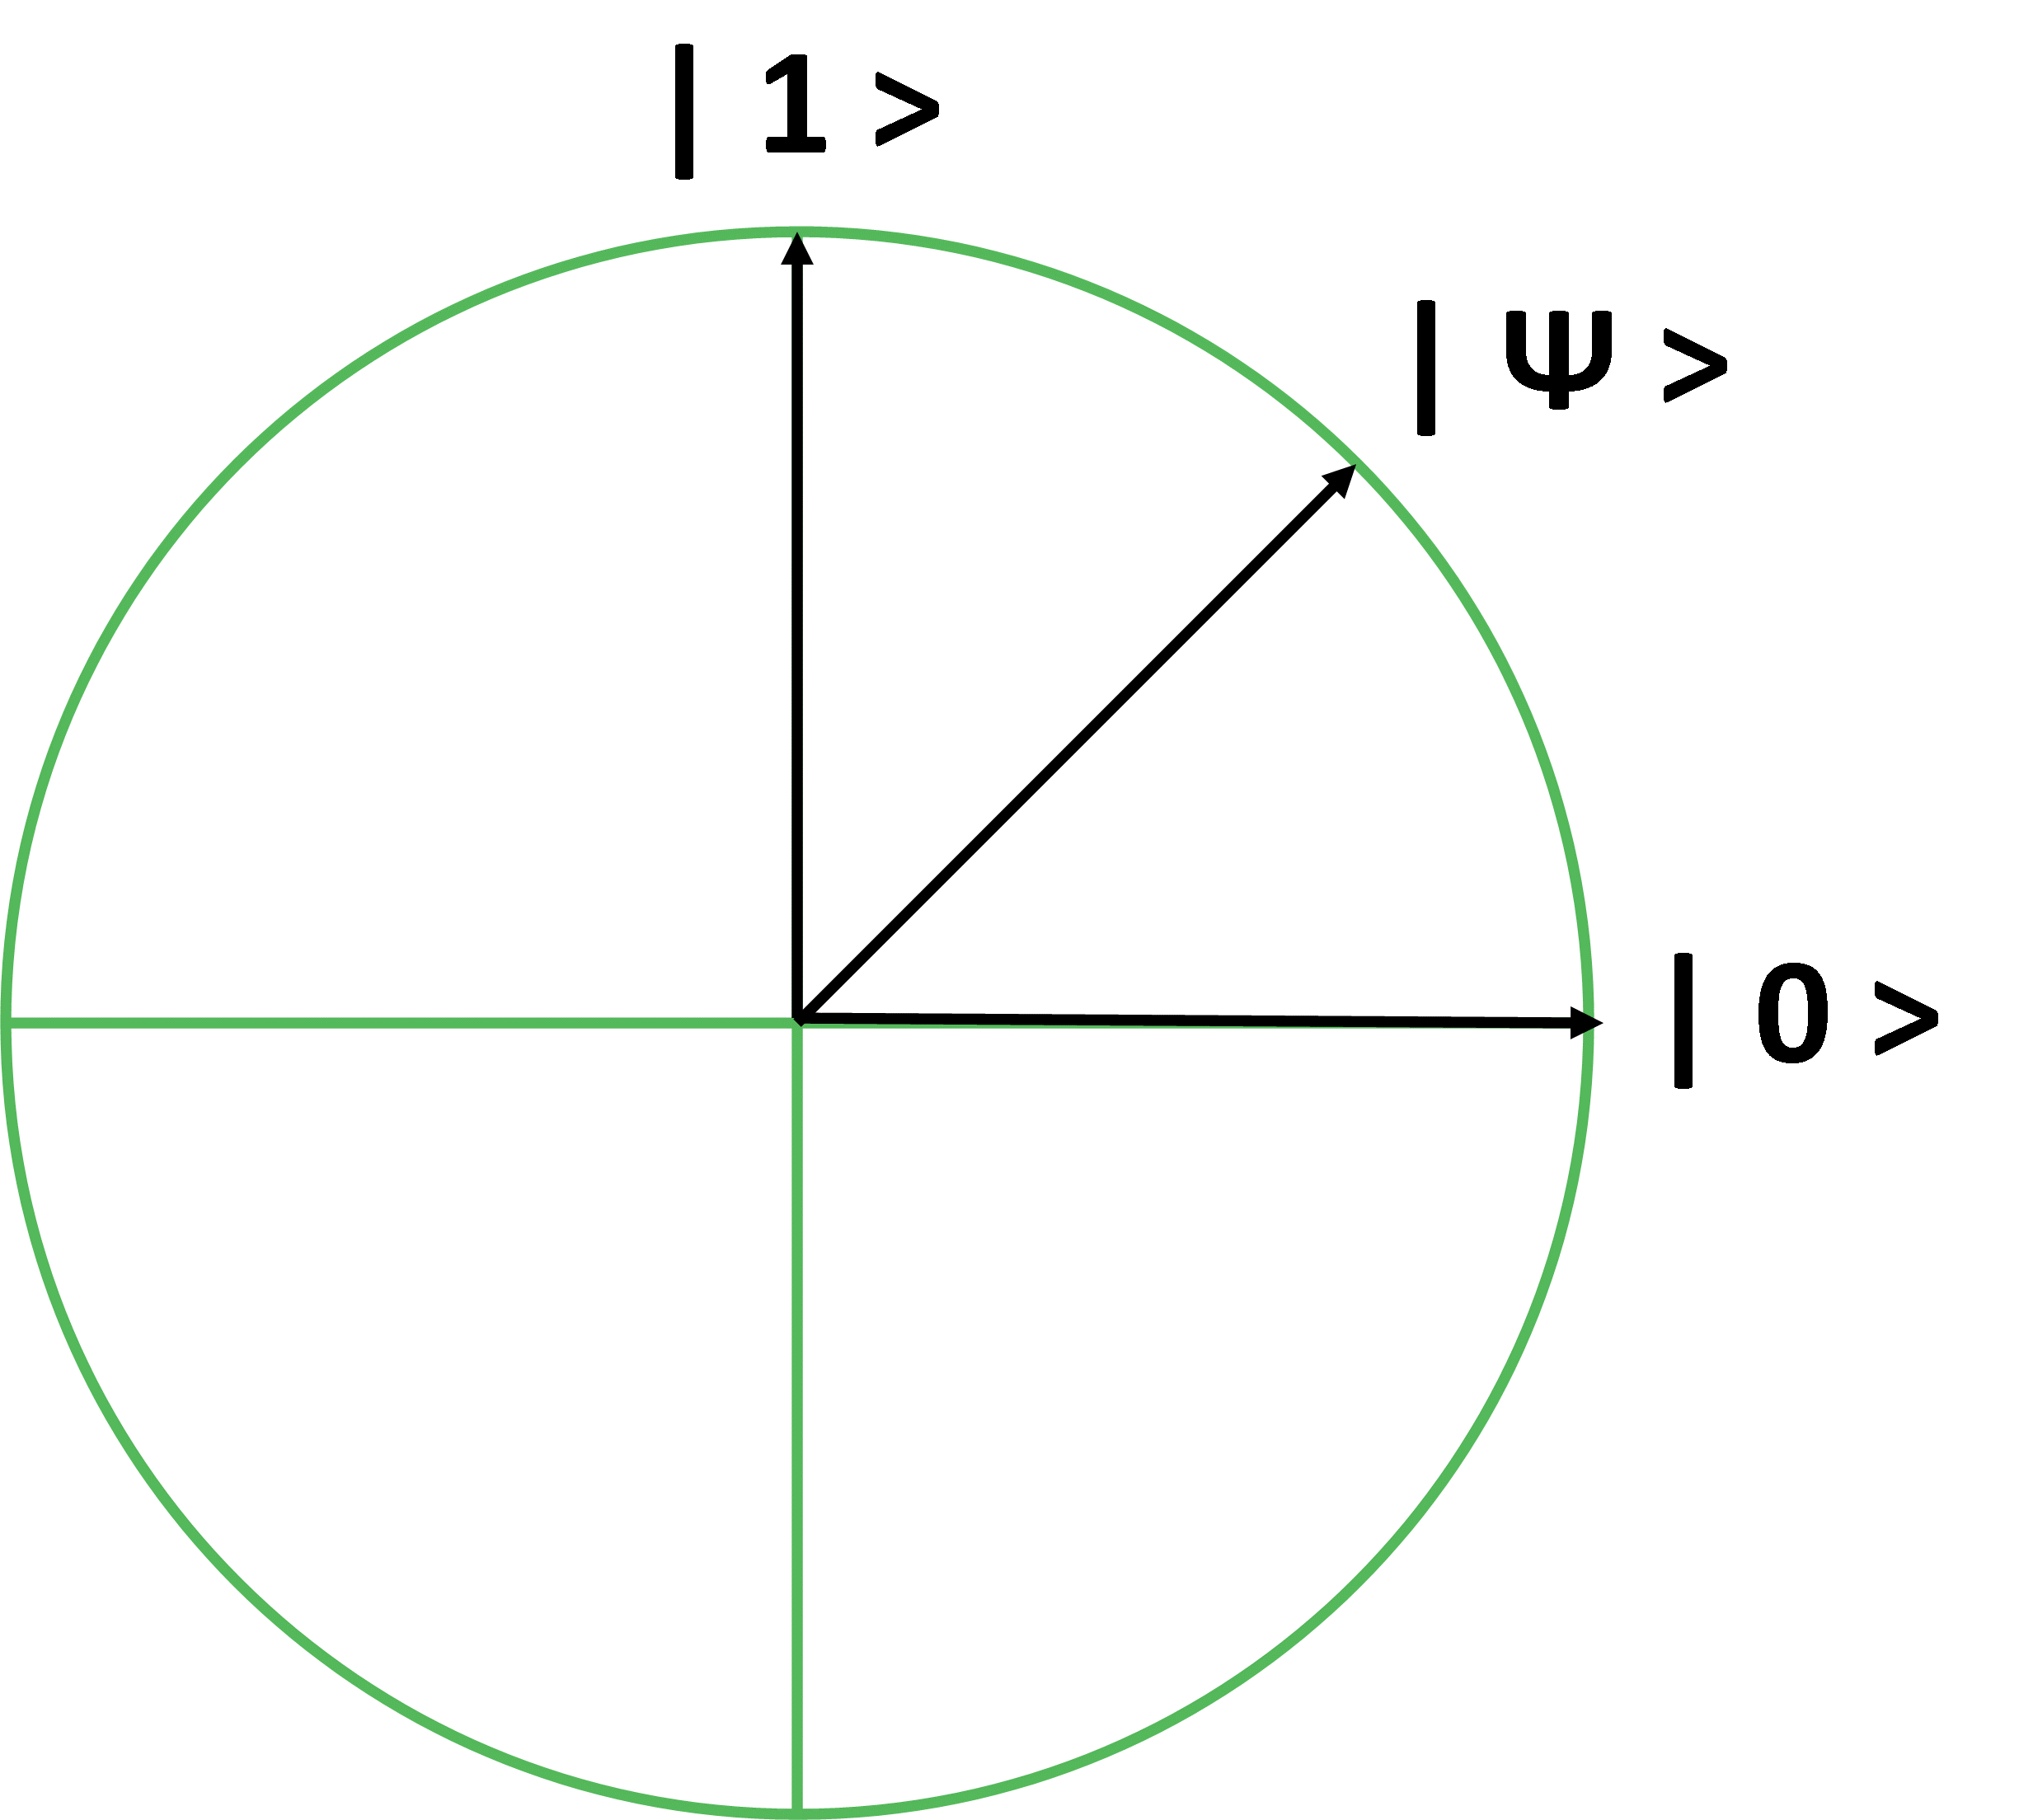
\includegraphics[width=0.8\linewidth]{img/qbit_thic} 
\end{center}

\noindent \textbf{Encryption key}: A secret sequence of characters that can be used with a program to scramble text in a unique way, so that it can only be unscrambled if you know the full sequence.\\

\noindent \textbf{Basis/bases}: Just as we can \textit{decompose}, or break-down, a line on a graph into a simple set of x- and y-coordinates, we can decompose polarisation into a combination of simple units, each called a "base", for instance "horizontal" or "vertical". A full set is called a "basis", plural "bases", which confusingly is spelled the same as the plural for "base", but pronounced "bay-sees".\\

\noindent \textbf{Qubit}: A 2D quantum system represented in the \textit{computational basis}. \\

\noindent \textbf{Bell Measurement}: A joint measurement performed on a two qubit state that expresses correlations between the qubits.

\end{multicols}

}

%%%%%%%%%%%%%%%%%%%%%%%%%%%%%%%%%%%%%%%%%%%%%%%%%%%%%%%%%%%%%%%%%%%%%%%%%%%%%%
  \headerbox{Measurement Device Independence}{name=Measurement Device Independence,column=1, span=2,below=Definitions, above=bottom}{
%%%%%%%%%%%%%%%%%%%%%%%%%%%%%%%%%%%%%%%%%%%%%%%%%%%%%%%%%%%%%%%%%%%%%%%%%%%%%%

\begin{multicols}{2}

\noindent Alice and Bob are sick of having their secrets discovered by Eve. Bobs been reading the newest issue of cryptographic weekly and discovers a new approach, \textbf{Measurement Device Independent Quantum Key Distribution}. Instead of sending their secrets directly to each other, they send them to a third party, there friend \textbf{Charlie}. Charlie can combine Alice and Bob's \textbf{information} and perform an operation unique to quantum physics, called a \textbf{Bell Measurement}. The bell measurement provides a vital piece of information that when combined with Alice and Bob's data, allows them to work out what is being sent. As only Alice/Bob knows her/his outgoing data, only they can know what information is being passed through the network.

\vspace{0.3cm}

\noindent In celebration of finally having a secure network, Bob has had one too many pints and can no longer remember what he sent to Alice. Just like Eve, Bob is now locked out of the network, as he can no longer work out what Alice is sending him. Silly forgetful Bob!  

\begin{center}
    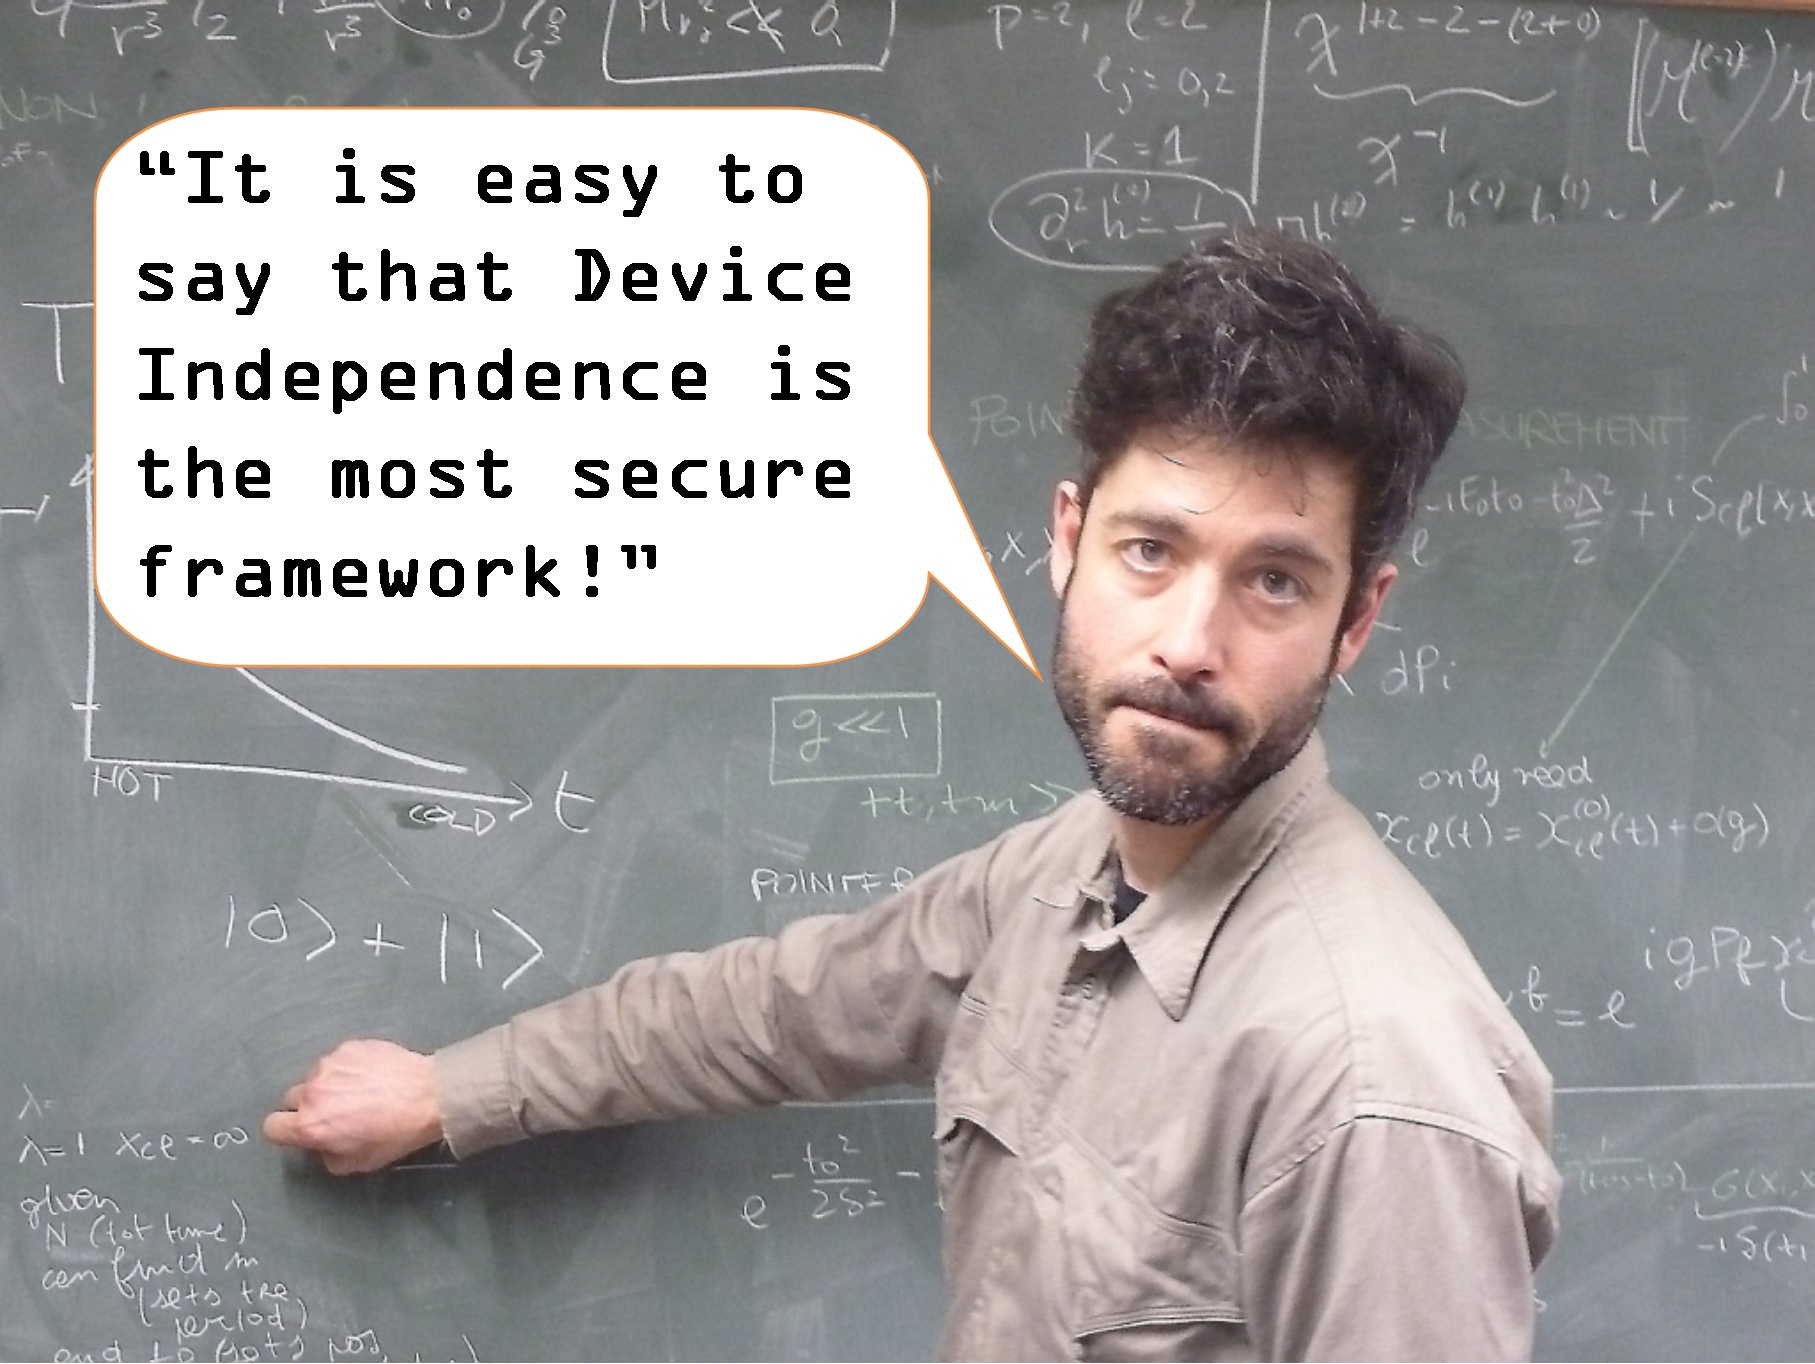
\includegraphics[width=\linewidth]{img/luis_sp} 
\end{center} 

\centering\textit{Dr Lluis Masanes - MDI Expert at UCL}

\end{multicols}
}



\end{poster}

\end{document}

